\documentclass[10pt]{article}

\usepackage[
  paperwidth=420mm,
  paperheight=594mm,
  margin=0mm
]{geometry}
\usepackage{fontspec}
\usepackage{xcolor}
\usepackage{graphicx}
\usepackage{tikz}
\usepackage{ragged2e}

\usetikzlibrary{arrows.meta, calc, positioning}

\setmainfont{texgyreheros-regular.otf}[
  Path = fonts/,
  BoldFont = texgyreheros-bold.otf,
  ItalicFont = texgyreheros-italic.otf,
  BoldItalicFont = texgyreheros-bolditalic.otf
]
\setsansfont{texgyreheros-regular.otf}[
  Path = fonts/,
  BoldFont = texgyreheros-bold.otf,
  ItalicFont = texgyreheros-italic.otf,
  BoldItalicFont = texgyreheros-bolditalic.otf
]

\definecolor{Page}{HTML}{F6F8FA}
\definecolor{Navy}{HTML}{102F46}
\definecolor{DeepNavy}{HTML}{082033}
\definecolor{Teal}{HTML}{0F7B78}
\definecolor{Gold}{HTML}{D79322}
\definecolor{Ink}{HTML}{1F2933}
\definecolor{Slate}{HTML}{586A78}
\definecolor{Line}{HTML}{CED9DF}
\definecolor{SoftBlue}{HTML}{EAF2F7}
\definecolor{SoftTeal}{HTML}{E6F3F2}
\definecolor{SoftGold}{HTML}{FFF3D9}
\definecolor{SoftRed}{HTML}{FFF0EA}
\definecolor{SoftGray}{HTML}{EEF2F4}

\pagestyle{empty}
\setlength{\parindent}{0pt}
\renewcommand{\familydefault}{\sfdefault}

\newcommand{\heading}[1]{{\bfseries\fontsize{13.8}{16.2}\selectfont\color{Navy}#1}}
\newcommand{\subheading}[1]{{\bfseries\fontsize{9.2}{11.0}\selectfont\color{Ink}#1}}
\newcommand{\bodytext}{\fontsize{8.2}{9.8}\selectfont\color{Ink}}
\newcommand{\tinytext}{\fontsize{6.4}{7.8}\selectfont\color{Slate}}
\newcommand{\tagtext}{\fontsize{6.7}{8.0}\selectfont\color{Ink}}
\newcommand{\metricnum}{\bfseries\fontsize{18}{20}\selectfont\color{DeepNavy}}
\newcommand{\metriclabel}{\bfseries\fontsize{7.1}{8.3}\selectfont\color{Ink}}

\begin{document}
\begin{tikzpicture}[remember picture, overlay, x=1mm, y=-1mm]
\coordinate (O) at (current page.north west);
\begin{scope}[shift={(O)}]

% Background
\fill[Page] (0,0) rectangle (420,594);

% Header
\draw[fill=Navy, draw=Navy, rounded corners=2.5mm] (12,12) rectangle (408,62);
\node[anchor=north west, inner sep=0pt] at (22,19)
  {\colorbox{white}{
\includegraphics[height=34mm]{images/ganesha.jpg}}};
\node[anchor=north west, text width=255mm, inner sep=0pt] at (64,18) {
  {\bfseries\fontsize{24.2}{27.5}\selectfont\color{white}
  Perancangan Arsitektur Sistem Otomasi Inspeksi Kontainer\\[-0.5mm]di Pelabuhan}\par
  \vspace{2mm}
  {\fontsize{10.8}{13}\selectfont\color{white}
  Aththariq Lisan Quran Daulah Sentono \;|\; 18222013 \;|\; Sistem dan Teknologi Informasi, ITB}\par
  \vspace{1mm}
  {\fontsize{8.5}{10.5}\selectfont\color{white!80}
  Pembimbing: Ir. I Gusti Bagus Baskara Nugraha, S.T., M.T., Ph.D}
};
\node[anchor=north east, inner sep=0pt] at (396,23) {
  \begin{minipage}{54mm}
  \raggedleft
  {\bfseries\fontsize{12.5}{14}\selectfont\color{Gold}Tugas Akhir}\par
  {\fontsize{10}{12}\selectfont\color{white}Cargovision}\par
  \vspace{1mm}
  {\fontsize{7.5}{9}\selectfont\color{white!72}A2 portrait}
  \end{minipage}
};

% Narrative strip
\draw[fill=white, draw=Line, rounded corners=2.2mm] (12,70) rectangle (408,94);
\node[anchor=west, inner sep=0pt, text width=82mm] at (22,82) {
  {\bfseries\fontsize{9.4}{11}\selectfont\color{Slate}Kondisi awal}\par
  {\fontsize{8.2}{9.8}\selectfont\color{Ink}Pencatatan dan bukti inspeksi tersebar}
};
\draw[-{Latex[length=3mm]}, line width=0.9pt, draw=Teal] (113,82) -- (151,82);
\node[anchor=west, inner sep=0pt, text width=102mm] at (160,82) {
  {\bfseries\fontsize{10.4}{12}\selectfont\color{Navy}Gagasan rancangan}\par
  {\fontsize{8.3}{9.8}\selectfont\color{Ink}Kontainer menjadi pusat riwayat inspeksi}
};
\draw[-{Latex[length=3mm]}, line width=0.9pt, draw=Teal] (269,82) -- (307,82);
\node[anchor=west, inner sep=0pt, text width=84mm] at (316,82) {
  {\bfseries\fontsize{9.4}{11}\selectfont\color{Slate}Hasil evaluasi}\par
  {\fontsize{8.2}{9.8}\selectfont\color{Ink}Kebutuhan dipetakan ke arsitektur dan skenario kapasitas}
};

% Hero architecture card
\draw[fill=white, draw=Line, rounded corners=3mm] (12,103) rectangle (408,315);
\node[anchor=north west, inner sep=0pt] at (22,113) {\heading{Arsitektur Cargovision Berpusat pada Kontainer}};
\draw[draw=Teal, line width=0.6pt] (22,130) -- (398,130);

% Layer backgrounds
\draw[fill=SoftBlue, draw=Teal!20, rounded corners=3mm] (24,142) rectangle (105,292);
\draw[fill=SoftTeal, draw=Teal!22, rounded corners=3mm] (119,142) rectangle (214,292);
\draw[fill=SoftGold, draw=Gold!26, rounded corners=3mm] (228,142) rectangle (314,292);
\draw[fill=SoftGray, draw=Slate!22, rounded corners=3mm] (326,142) rectangle (396,292);
\node[anchor=north west] at (30,147) {\tinytext\bfseries Edge Layer};
\node[anchor=north west] at (125,147) {\tinytext\bfseries Application \& Web};
\node[anchor=north west] at (234,147) {\tinytext\bfseries Data Layer};
\node[anchor=north west] at (332,147) {\tinytext\bfseries Sistem eksternal};

% Node styles as manual rectangles
\tikzset{
  archarrow/.style={-{Latex[length=2.4mm,width=1.7mm]}, draw=Navy, line width=0.75pt},
  livearrow/.style={-{Latex[length=2.4mm,width=1.7mm]}, draw=Teal, line width=0.75pt, dashed},
  extarrow/.style={-{Latex[length=2.4mm,width=1.7mm]}, draw=Slate, line width=0.72pt, dashed}
}

% Left image hint
\node[anchor=north west, inner sep=0pt] at (32,161)
  {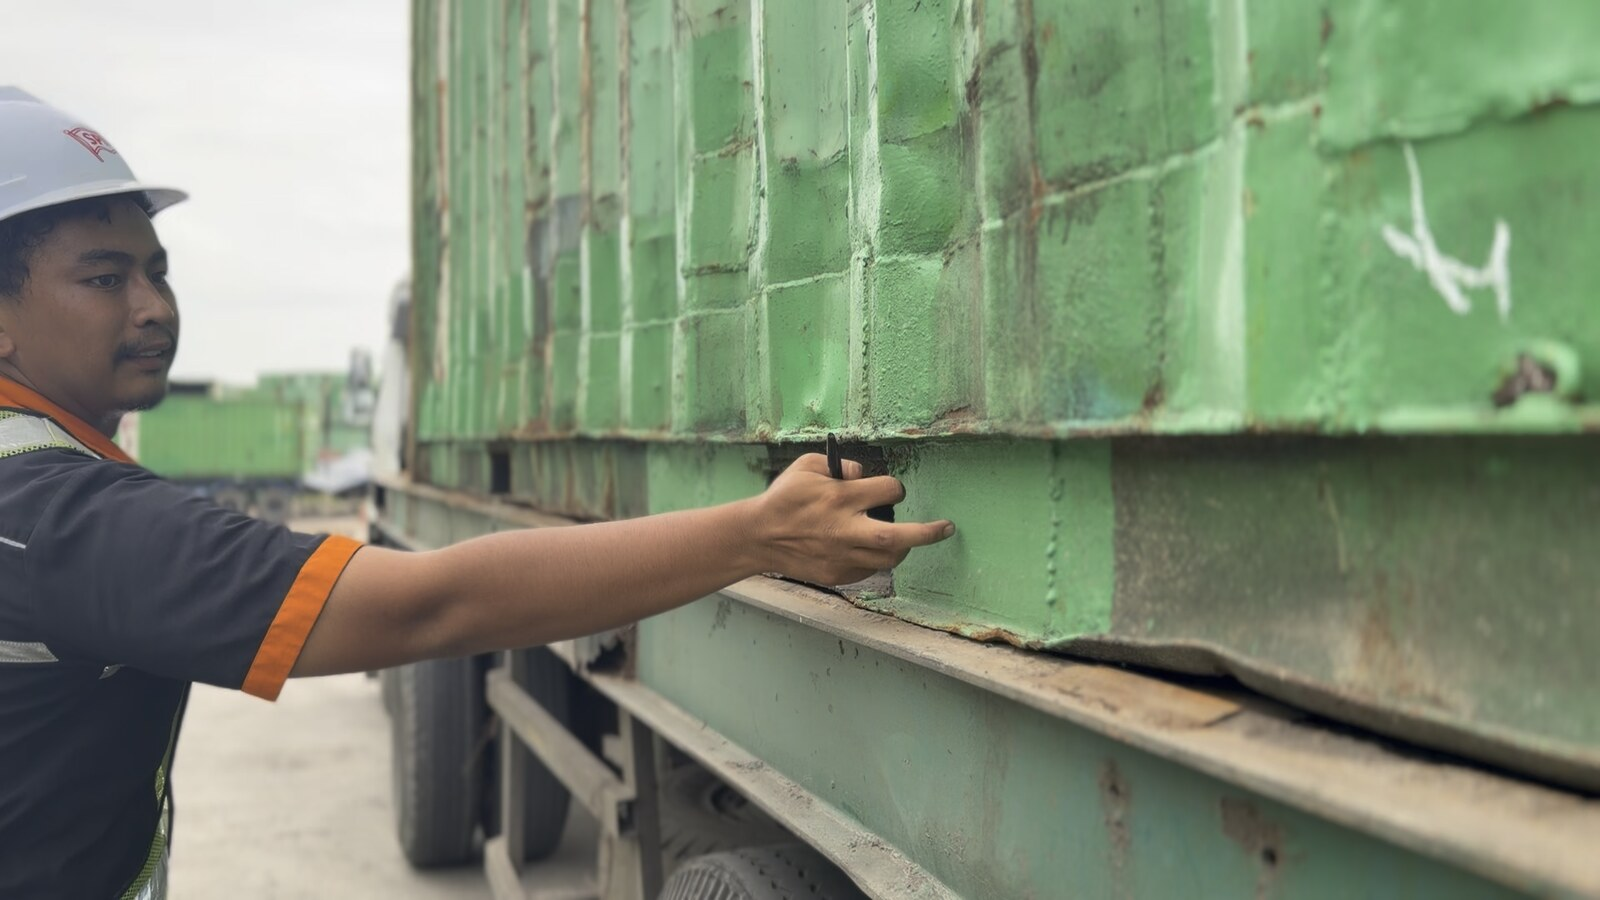
\includegraphics[width=63mm,height=35mm,keepaspectratio]{images/evidence-eksisting-inspeksi-fisik.jpg}};
\node[anchor=north west, text width=64mm, align=center] at (32,197)
  {\tinytext Bukti lapangan: inspeksi kontainer};

% Architecture nodes
\draw[fill=white, draw=Slate, rounded corners=2.1mm, line width=0.65pt] (36,212) rectangle (94,234);
\node[align=center] at (65,223) {\subheading{Kamera RTSP}\\[-0.4mm]{\tinytext akuisisi video}};
\draw[fill=white, draw=Slate, rounded corners=2.1mm, line width=0.65pt] (34,246) rectangle (96,276);
\node[align=center] at (65,261) {\subheading{Cargovision Edge}\\[-0.2mm]{\fontsize{8.2}{9.5}\selectfont OCR dan pemindaian visual}};

\draw[fill=white, draw=Slate, rounded corners=2.1mm, line width=0.65pt] (135,160) rectangle (198,188);
\node[align=center] at (166.5,174) {\subheading{API Cargovision}\\[-0.3mm]{\tinytext orkestrasi dan validasi}};
\draw[fill=Gold!18, draw=Gold!80!black, rounded corners=2.4mm, line width=0.95pt] (128,207) rectangle (205,249);
\node[align=center] at (166.5,228) {{\bfseries\fontsize{11.4}{13}\selectfont\color{DeepNavy}Kontainer}\\[-0.2mm]{\fontsize{8.4}{10}\selectfont\color{Ink}pusat riwayat inspeksi}};
\draw[fill=white, draw=Slate, rounded corners=2.1mm, line width=0.65pt] (136,268) rectangle (197,288);
\node[align=center] at (166.5,278) {\subheading{Aplikasi Web}};

\draw[fill=white, draw=Slate, rounded corners=2.1mm, line width=0.65pt] (243,160) rectangle (300,183);
\node[align=center] at (271.5,171.5) {\subheading{MongoDB}\\[-0.4mm]{\tinytext data terstruktur}};
\draw[fill=white, draw=Slate, rounded corners=2.1mm, line width=0.65pt] (243,207) rectangle (300,230);
\node[align=center] at (271.5,218.5) {\subheading{R2}\\[-0.4mm]{\tinytext artefak visual}};
\draw[fill=white, draw=Slate, rounded corners=2.1mm, line width=0.65pt] (243,254) rectangle (300,277);
\node[align=center] at (271.5,265.5) {\subheading{Audit}\\[-0.4mm]{\tinytext waktu dan aktor}};

\draw[fill=white, draw=Slate, rounded corners=1.8mm, dashed, line width=0.6pt] (337,160) rectangle (386,181);
\node[align=center] at (361.5,170.5) {\subheading{TOS/PCS}};
\draw[fill=white, draw=Slate, rounded corners=1.8mm, dashed, line width=0.6pt] (337,193) rectangle (386,214);
\node[align=center] at (361.5,203.5) {\subheading{Inaportnet}};
\draw[fill=white, draw=Slate, rounded corners=1.8mm, dashed, line width=0.6pt] (337,226) rectangle (386,247);
\node[align=center] at (361.5,236.5) {\subheading{Bea Cukai}};
\draw[fill=white, draw=Slate, rounded corners=2.1mm, line width=0.65pt] (332,265) rectangle (391,287);
\node[align=center] at (361.5,276) {\subheading{Integration}\\[-0.4mm]{\tinytext kesiapan perluasan}};

% Architecture arrows
\draw[archarrow] (65,234) -- (65,246);
\draw[archarrow] (96,261) -- node[above, fill=white, inner sep=1pt] {\tinytext HTTP} (135,174);
\draw[archarrow] (166.5,188) -- (166.5,207);
\draw[archarrow] (166.5,249) -- (166.5,268);
\draw[archarrow] (205,228) -- node[above, fill=white, inner sep=1pt] {\tinytext riwayat} (243,218.5);
\draw[archarrow] (198,174) -- ++(18,0) |- (243,171.5);
\draw[archarrow] (198,174) -- ++(14,0) |- (243,265.5);
\draw[livearrow] (65,276) -- ++(0,16) -| node[pos=0.32, below, fill=white, inner sep=1pt] {\tinytext WebSocket} (166.5,288);
\draw[extarrow] (337,170.5) -- (314,170.5) |- (198,174);
\draw[extarrow] (337,203.5) -- (314,203.5) |- (198,174);
\draw[extarrow] (337,236.5) -- (314,236.5) |- (198,174);
\draw[extarrow] (332,276) -- (300,265.5);

% Legend
\draw[fill=white, draw=Line, rounded corners=1.8mm] (326,302) rectangle (396,311);
\draw[archarrow] (331,306.5) -- (342,306.5);
\node[anchor=west] at (344,306.5) {\tinytext data internal};
\draw[livearrow] (374,306.5) -- (385,306.5);
\node[anchor=west] at (387,306.5) {\tinytext live};

% Row cards: problem, decisions, metrics
\draw[fill=white, draw=Line, rounded corners=2.5mm] (12,326) rectangle (138,415);
\node[anchor=north west, inner sep=0pt, text width=114mm] at (22,336) {
  \heading{Masalah Eksisting}\par\vspace{3mm}
  {\bodytext
  \textbullet\ Dokumen dan formulir masih muncul sebagai kertas atau input manual.\par
  \textbullet\ Identitas, hasil pemeriksaan, dan bukti visual belum selalu terhubung pada satu riwayat.\par
  \textbullet\ Integrasi eksternal perlu dibuat sebagai kontrak layanan, bukan klaim sambungan penuh.}
};
\draw[fill=SoftGray, draw=Line, rounded corners=1.5mm] (22,392) rectangle (128,407);
\node[anchor=north west, text width=98mm, inner sep=0pt] at (26,395) {
  {\tagtext\bfseries Fakta lapangan:} {\tagtext inspeksi fisik, dokumen kertas, dan input manual masih muncul.}
};

\draw[fill=white, draw=Line, rounded corners=2.5mm] (147,326) rectangle (273,415);
\node[anchor=north west, inner sep=0pt, text width=114mm] at (157,336) {
  \heading{Keputusan Rancangan}\par\vspace{3mm}
  {\bodytext
  \textbullet\ Edge menangani video, OCR, dan pemindaian awal dekat kamera.\par
  \textbullet\ API mengatur validasi, penyimpanan, autentikasi, dan orkestrasi.\par
  \textbullet\ Kontainer menjadi jangkar integrasi data inspeksi.\par
  \textbullet\ MongoDB dan R2 dipisahkan sesuai karakter data.}
};
\draw[fill=SoftGray, draw=Line, rounded corners=1.5mm] (157,392) rectangle (263,407);
\node[anchor=north west, text width=98mm, inner sep=0pt] at (161,395) {
  {\tagtext\bfseries Dampak:} {\tagtext aliran inspeksi dipetakan ke satu riwayat kontainer dan siap diintegrasikan.}
};

\draw[fill=white, draw=Line, rounded corners=2.5mm] (282,326) rectangle (408,415);
\node[anchor=north west, inner sep=0pt] at (292,336) {\heading{Evaluasi Kapasitas}};
\draw[fill=SoftTeal, draw=Teal!25, rounded corners=2mm] (292,354) rectangle (344,379);
\node[anchor=north west, inner sep=0pt] at (297,357) {\metricnum 96};
\node[anchor=north west, inner sep=0pt] at (319,358.5) {\metriclabel kont./jam};
\node[anchor=north west, inner sep=0pt] at (319,368.0) {\tinytext terbaik};
\draw[fill=SoftBlue, draw=Teal!18, rounded corners=2mm] (348,354) rectangle (400,379);
\node[anchor=north west, inner sep=0pt] at (353,357) {\metricnum 42};
\node[anchor=north west, inner sep=0pt] at (375,358.5) {\metriclabel kont./jam};
\node[anchor=north west, inner sep=0pt] at (375,368.0) {\tinytext nominal};
\draw[fill=SoftRed, draw=Gold!18, rounded corners=2mm] (292,384) rectangle (344,409);
\node[anchor=north west, inner sep=0pt] at (297,387) {\metricnum 15};
\node[anchor=north west, inner sep=0pt] at (319,388.5) {\metriclabel kont./jam};
\node[anchor=north west, inner sep=0pt] at (319,398.0) {\tinytext terburuk};
\draw[fill=SoftGold, draw=Gold!28, rounded corners=2mm] (348,384) rectangle (400,409);
\node[anchor=north west, inner sep=0pt] at (353,387) {\metricnum 168};
\node[anchor=north west, inner sep=0pt] at (381,388.5) {\metriclabel kont./jam};
\node[anchor=north west, inner sep=0pt] at (381,398.0) {\tinytext empat jalur};

% Data model card
\draw[fill=white, draw=Line, rounded corners=2.5mm] (12,424) rectangle (206,518);
\node[anchor=north west, inner sep=0pt] at (22,434) {\heading{Model Data Konseptual}};
\draw[draw=Teal, line width=0.5pt] (22,450) -- (196,450);
\draw[fill=Gold!18, draw=Gold!80!black, rounded corners=2mm, line width=0.8pt] (82,465) rectangle (136,490);
\node[align=center] at (109,477.5) {{\bfseries\fontsize{10.2}{12}\selectfont\color{DeepNavy}Kontainer}\\[-0.5mm]{\tinytext pusat data}};
\draw[fill=white, draw=Slate, rounded corners=1.8mm] (23,459) rectangle (62,479);
\node[align=center] at (42.5,469) {\tinytext OCR};
\draw[fill=white, draw=Slate, rounded corners=1.8mm] (23,490) rectangle (62,510);
\node[align=center] at (42.5,500) {\tinytext Tinjauan};
\draw[fill=white, draw=Slate, rounded corners=1.8mm] (79,501) rectangle (139,512);
\node[align=center] at (109,506.5) {\tinytext Artefak visual};
\draw[fill=white, draw=Slate, rounded corners=1.8mm] (156,459) rectangle (195,479);
\node[align=center] at (175.5,469) {\tinytext Pemindaian};
\draw[fill=white, draw=Slate, rounded corners=1.8mm] (156,490) rectangle (195,510);
\node[align=center] at (175.5,500) {\tinytext Audit};
\draw[-{Latex[length=2mm]}, draw=Navy, line width=0.55pt] (62,469) -- (82,475);
\draw[-{Latex[length=2mm]}, draw=Navy, line width=0.55pt] (62,500) -- (82,484);
\draw[-{Latex[length=2mm]}, draw=Navy, line width=0.55pt] (109,501) -- (109,490);
\draw[-{Latex[length=2mm]}, draw=Navy, line width=0.55pt] (156,469) -- (136,475);
\draw[-{Latex[length=2mm]}, draw=Navy, line width=0.55pt] (156,500) -- (136,484);
\node[anchor=north west, text width=174mm, inner sep=0pt] at (22,514) {\tinytext Riwayat inspeksi dibaca melalui identitas kontainer yang sama.};

% Evidence card
\draw[fill=white, draw=Line, rounded corners=2.5mm] (214,424) rectangle (408,518);
\node[anchor=north west, inner sep=0pt] at (224,434) {\heading{Bukti Realisasi Internal}};
\draw[draw=Teal, line width=0.5pt] (224,450) -- (398,450);
\node[anchor=north west, inner sep=0pt] at (224,458)
  {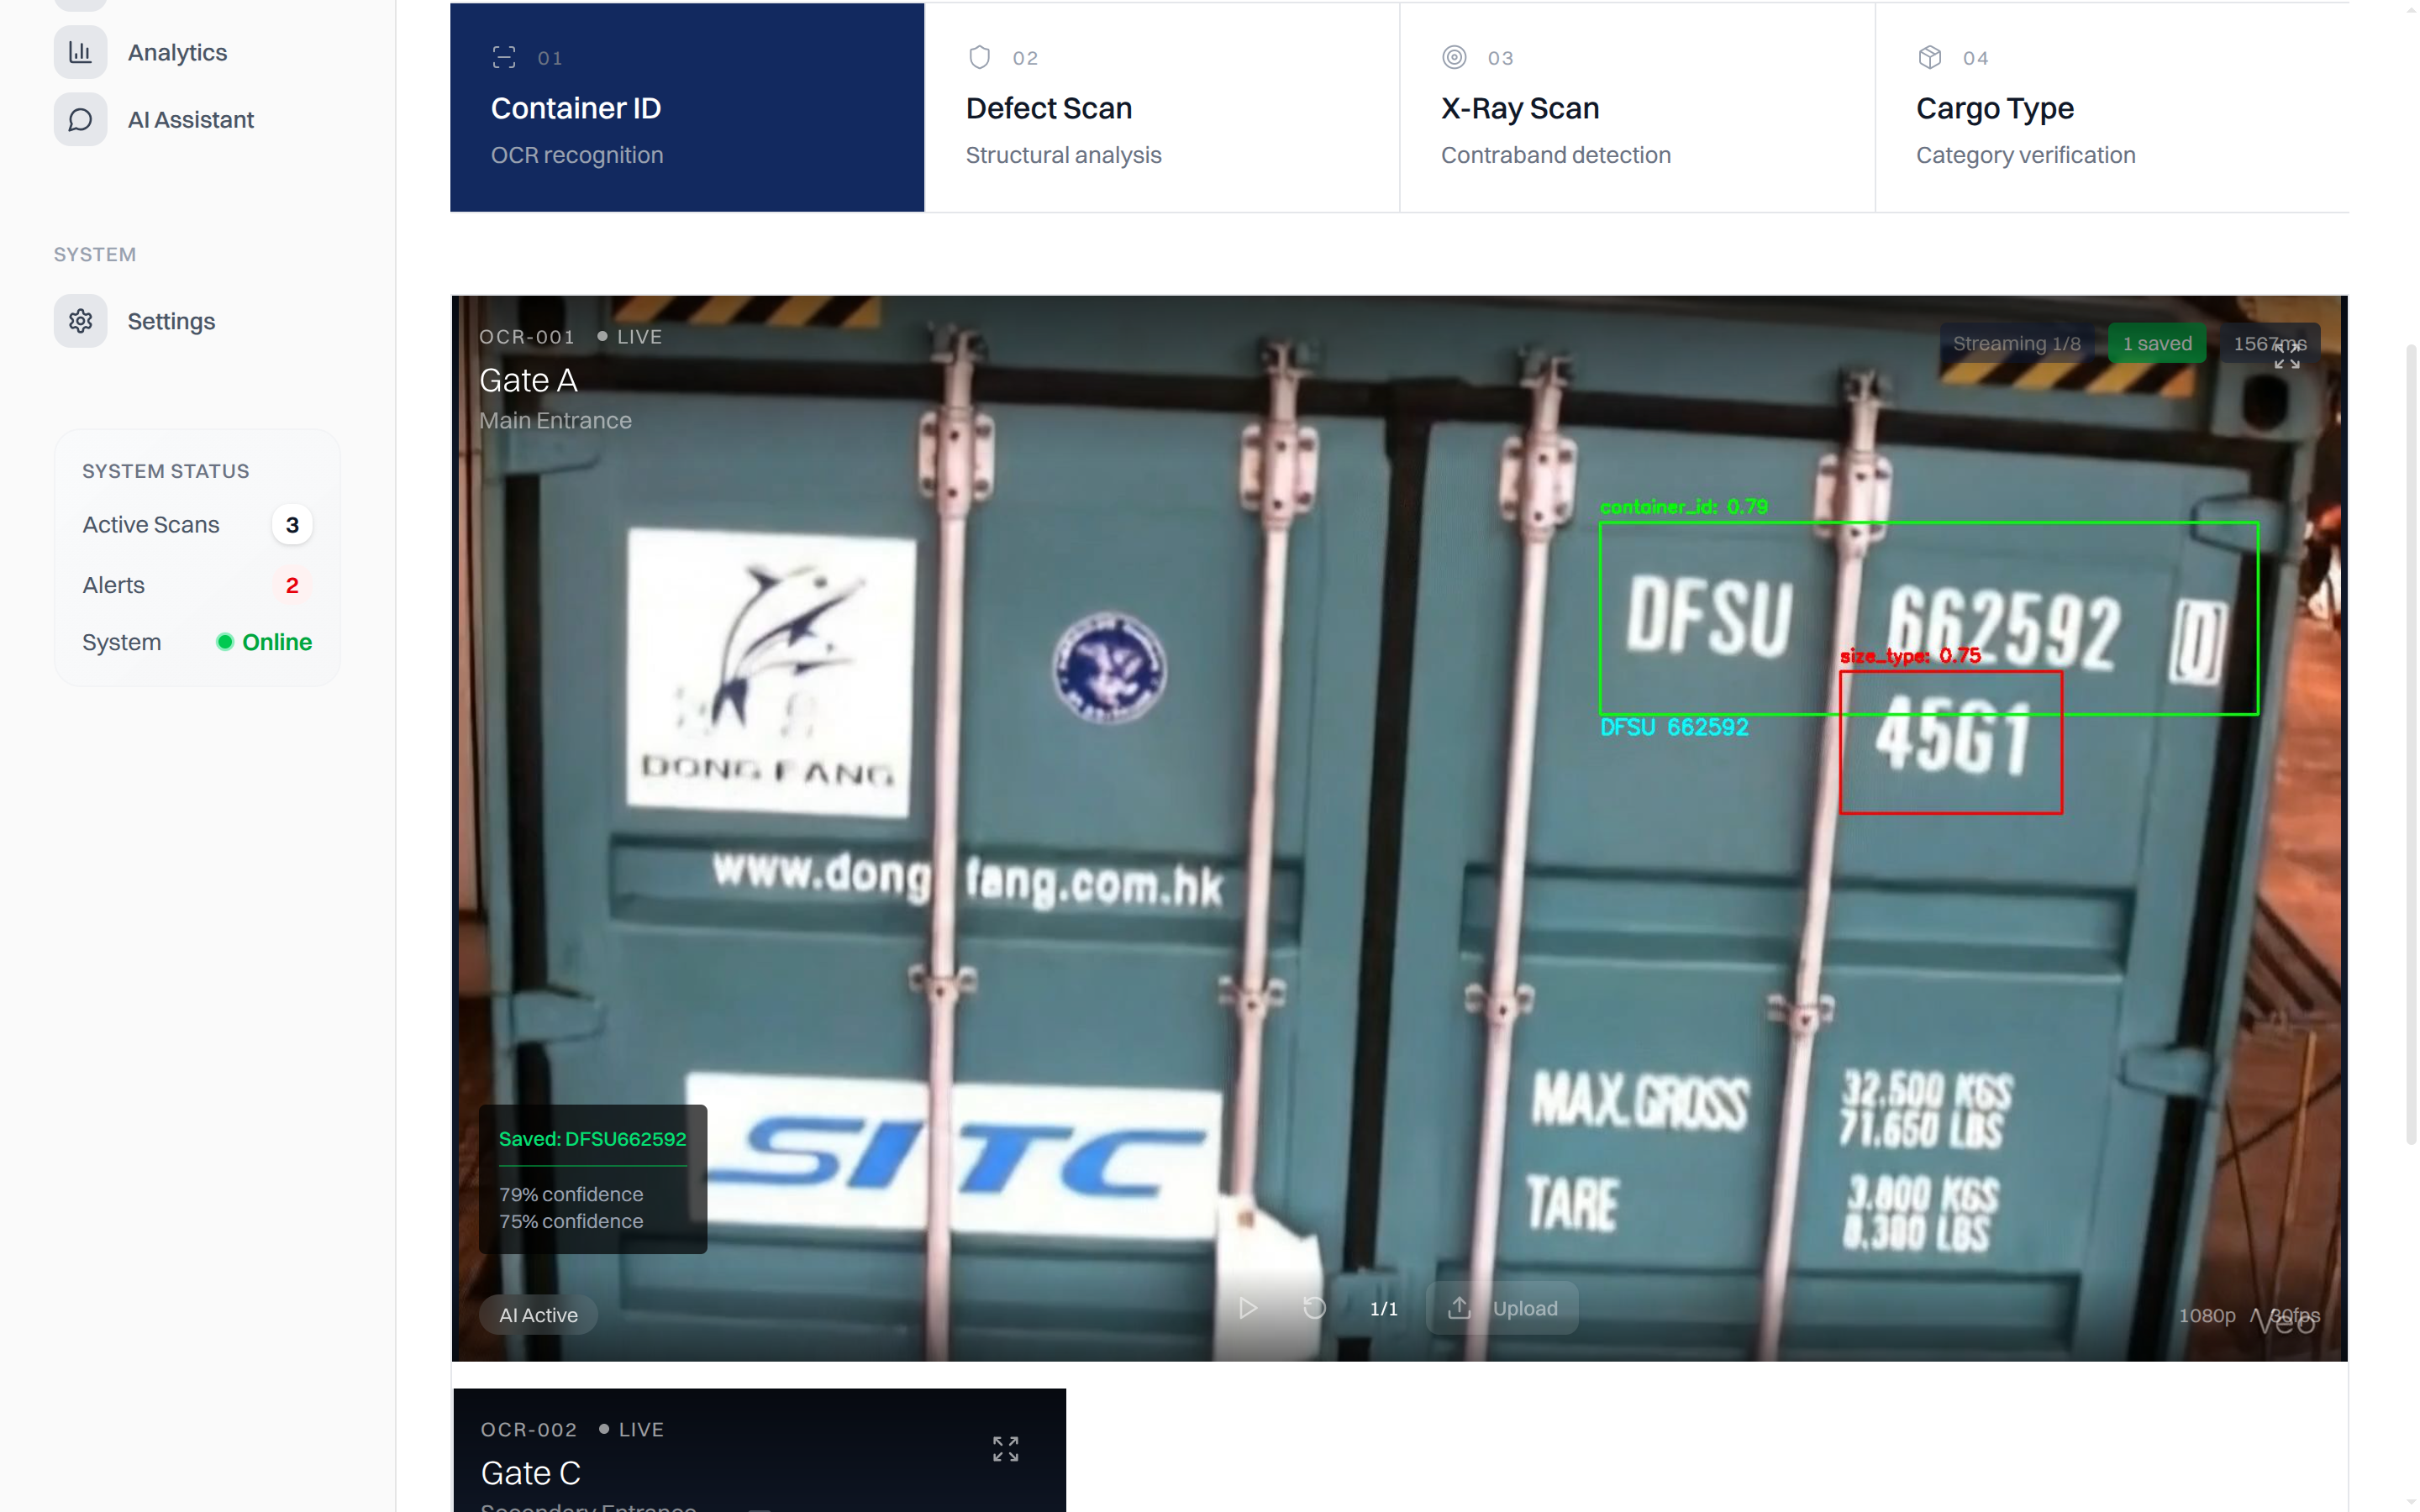
\includegraphics[width=40mm,height=25mm,keepaspectratio]{images/evidence-ocr-live.png}};
\node[anchor=north west, inner sep=0pt] at (266,458)
  {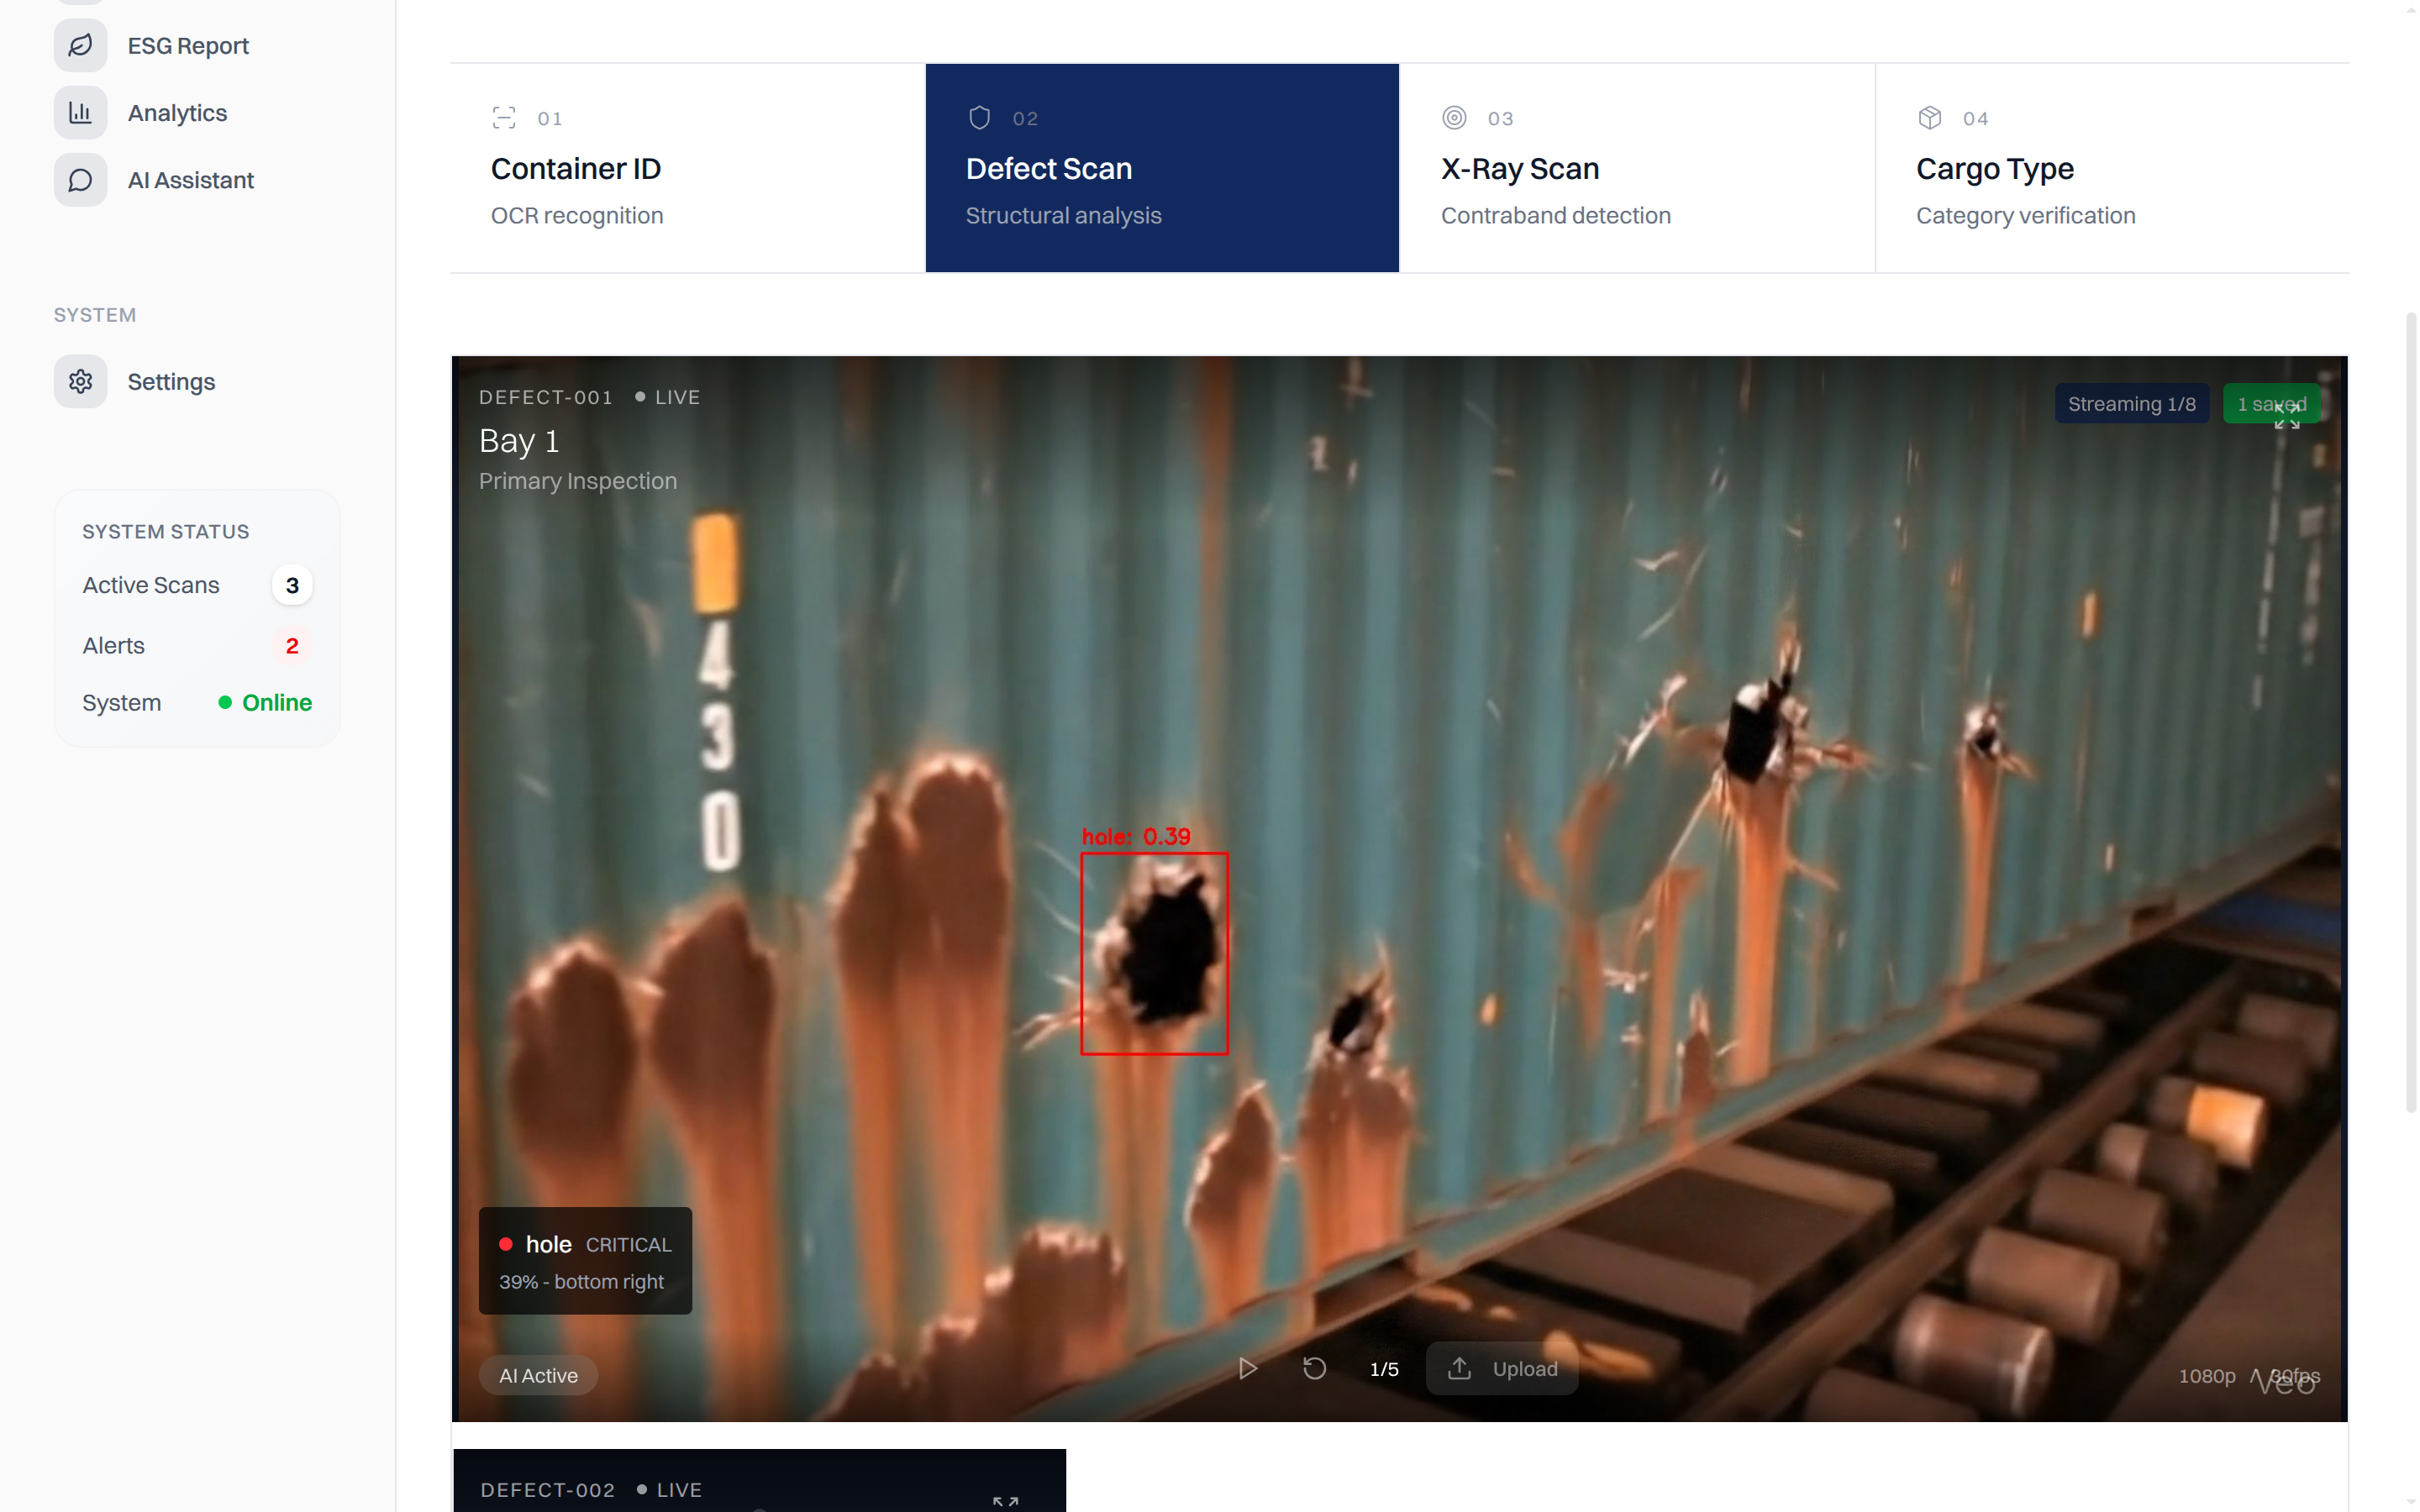
\includegraphics[width=40mm,height=25mm,keepaspectratio]{images/evidence-defect-live.png}};
\node[anchor=north west, inner sep=0pt] at (308,458)
  {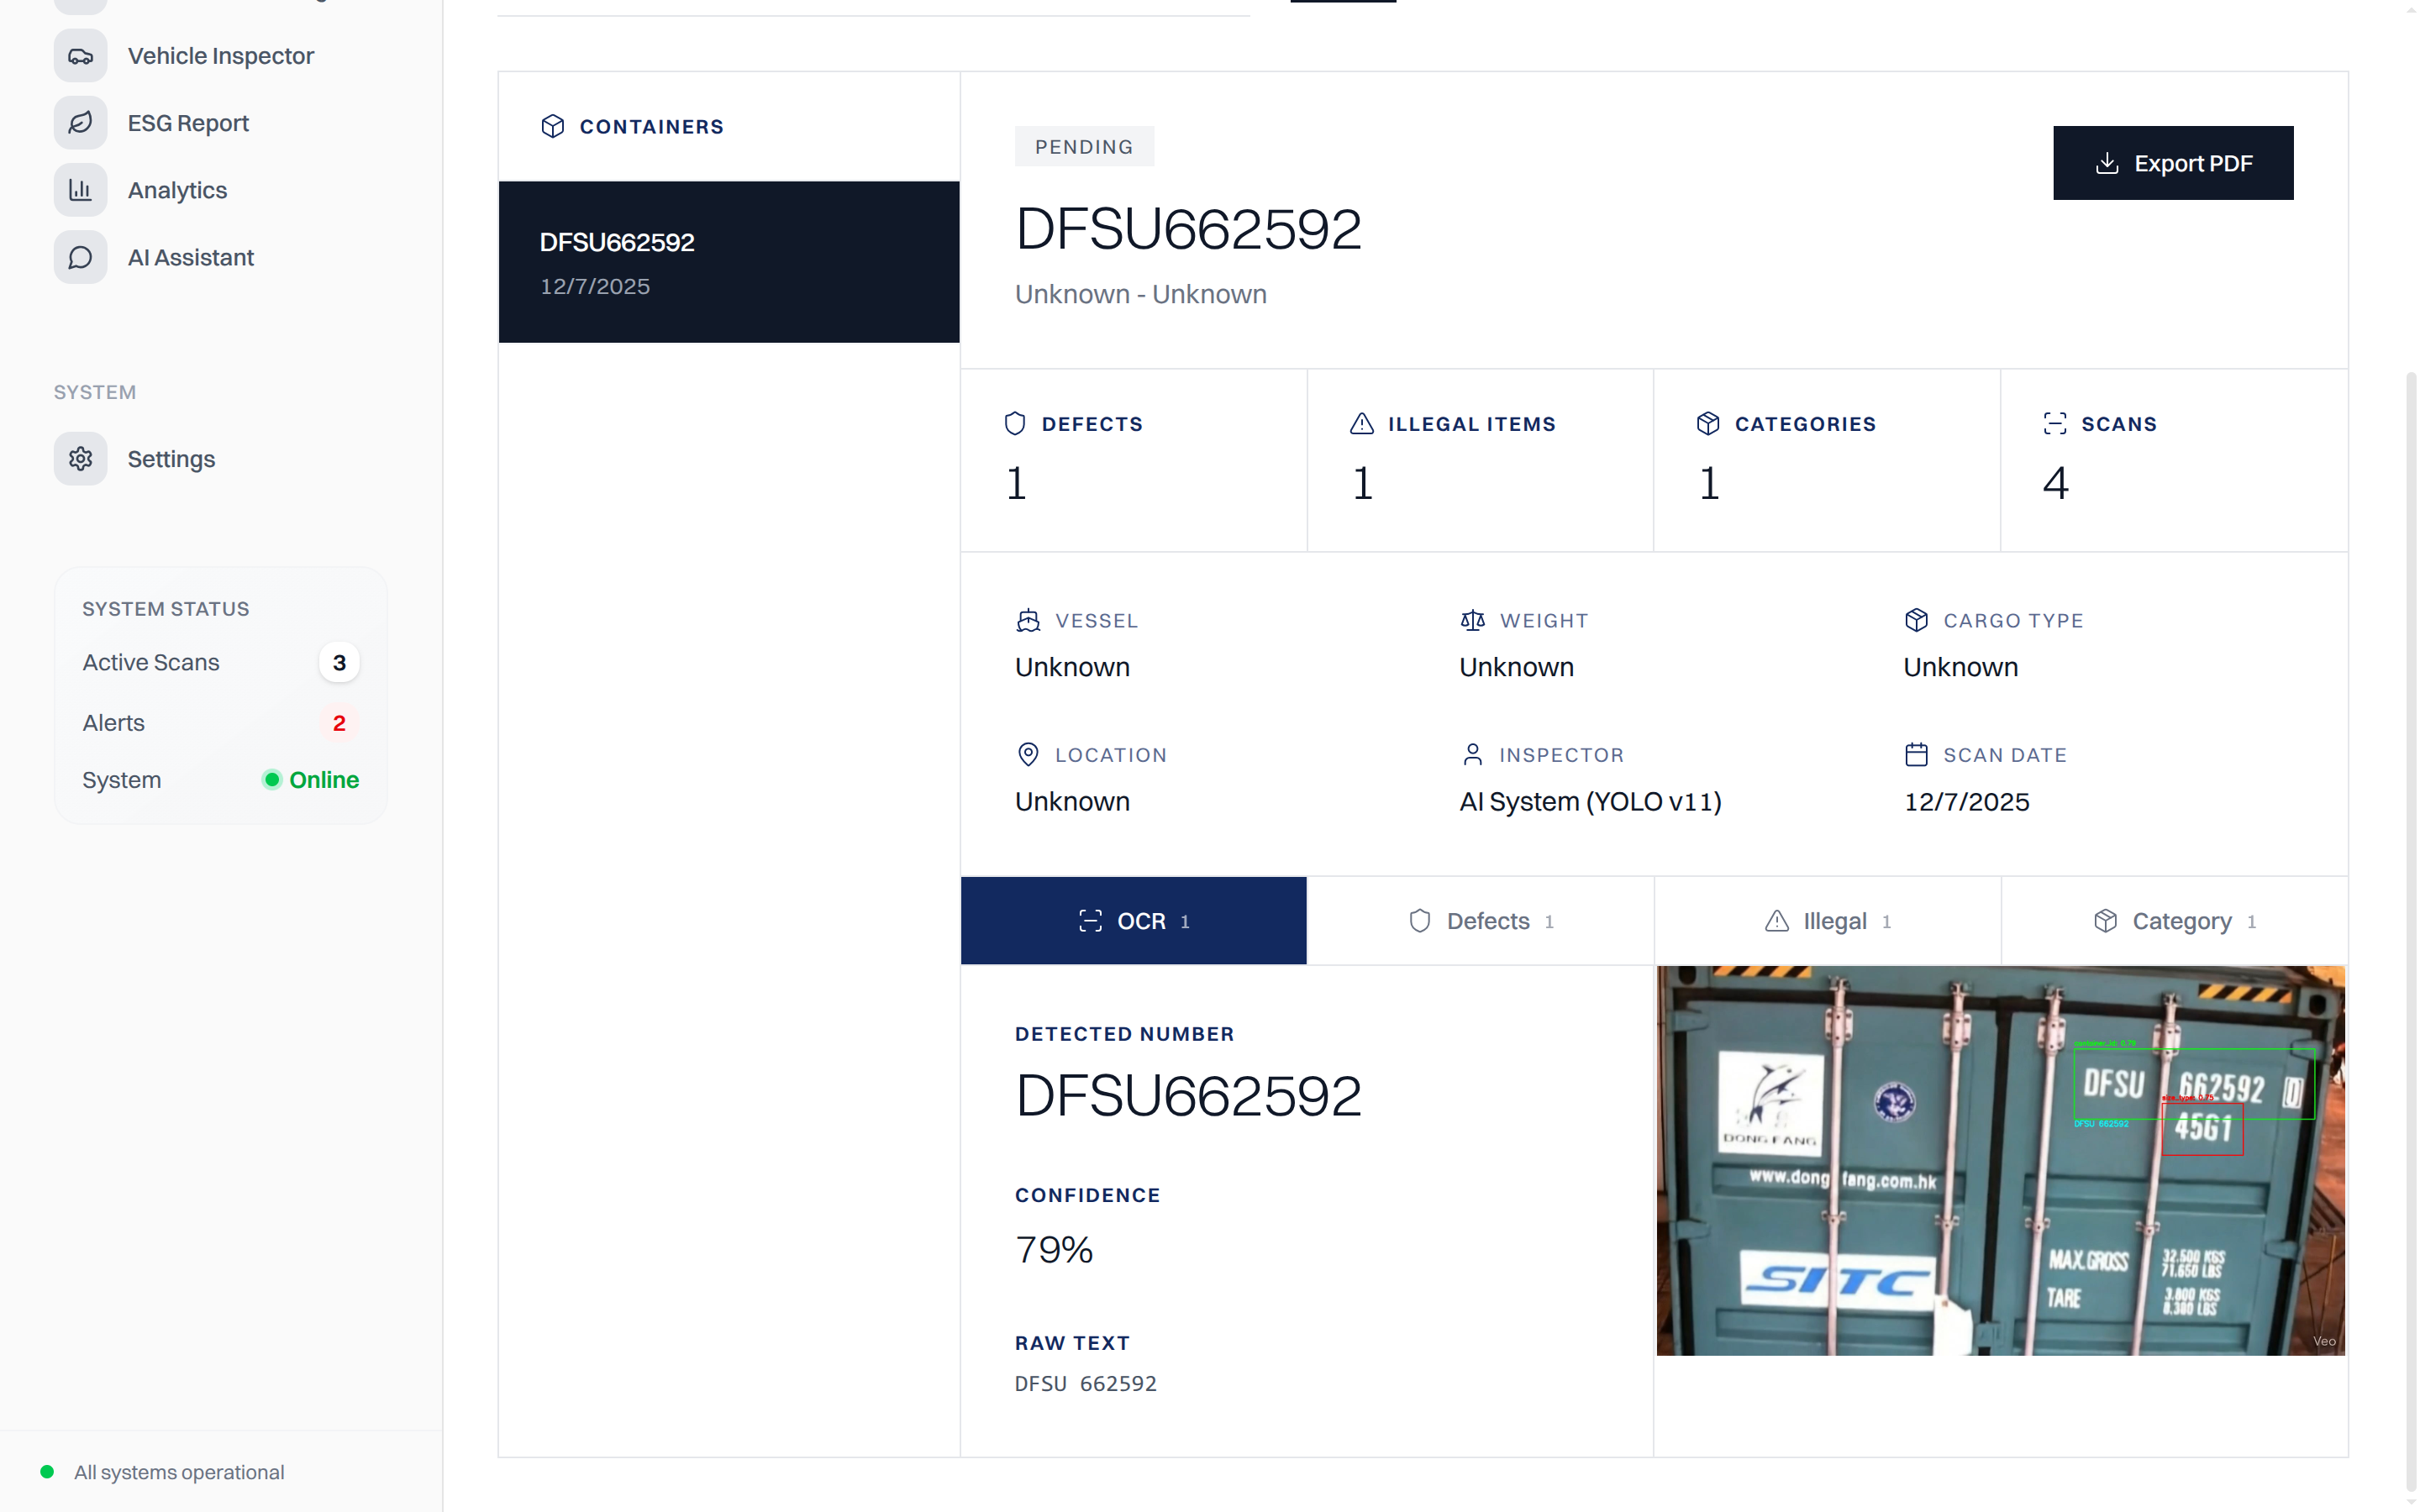
\includegraphics[width=40mm,height=25mm,keepaspectratio]{images/evidence-container-detail.png}};
\node[anchor=north west, inner sep=0pt] at (350,458)
  {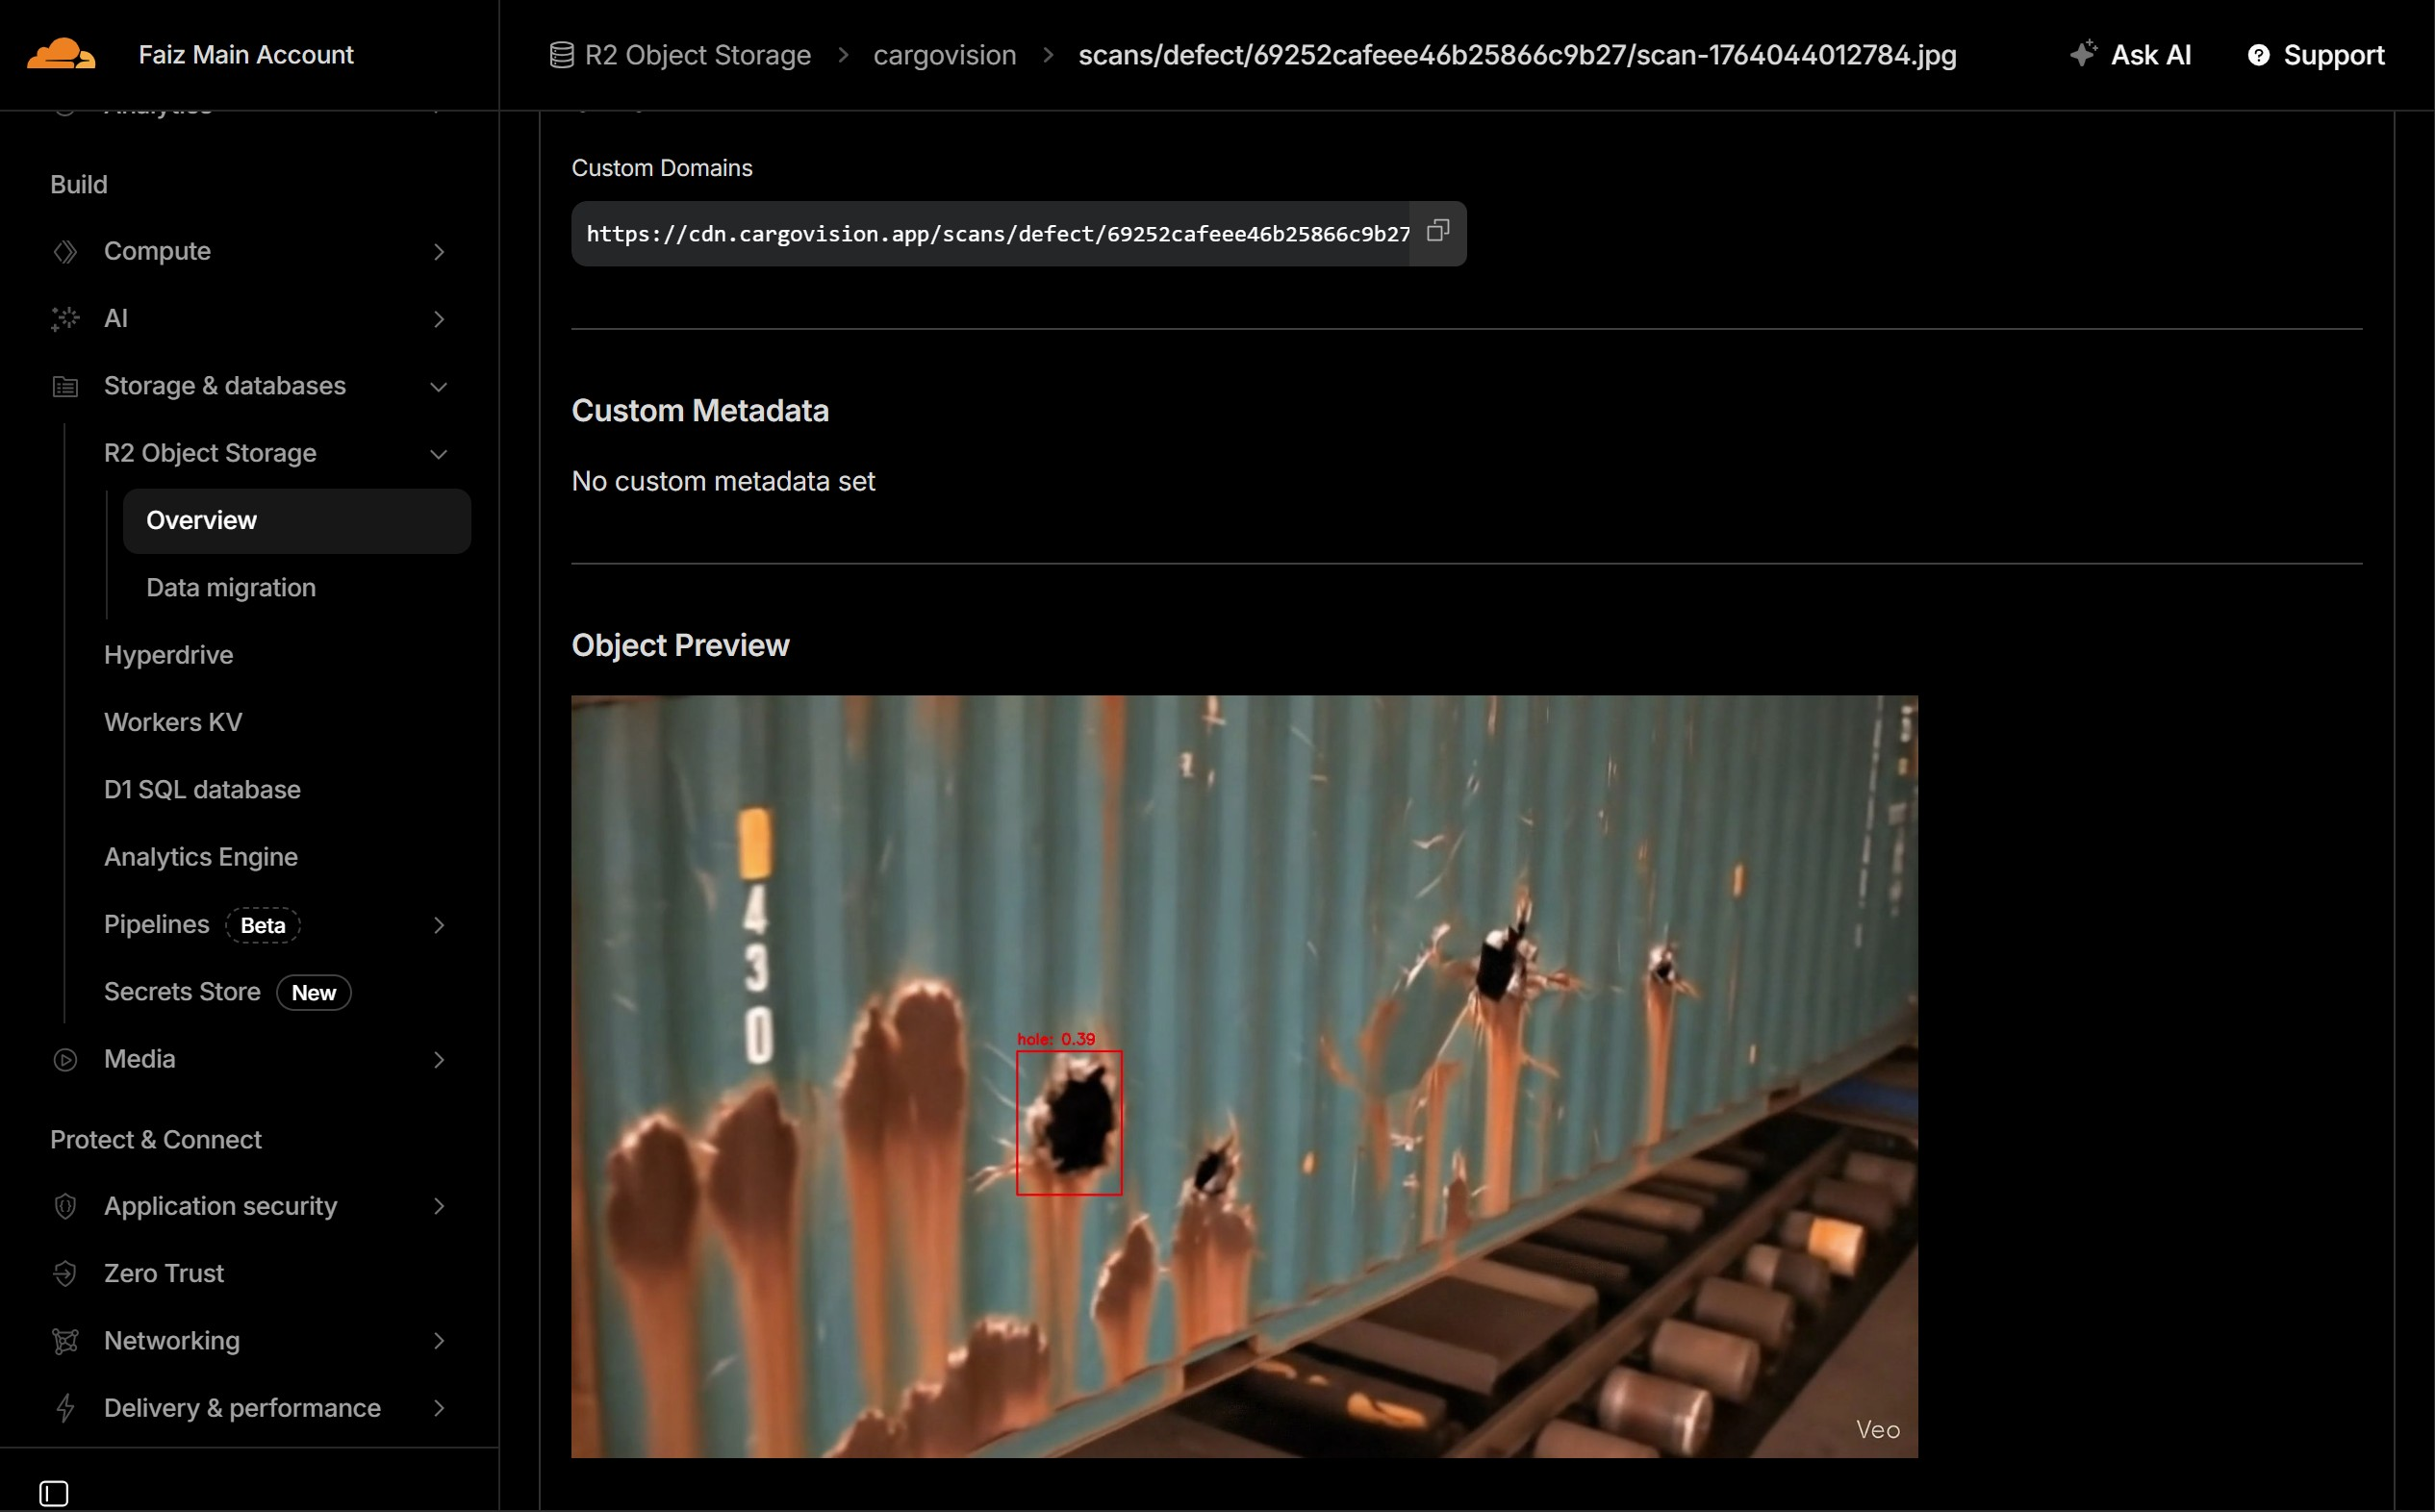
\includegraphics[width=40mm,height=25mm,keepaspectratio]{images/evidence-r2-storage.jpg}};
\node[anchor=north west, align=center, text width=40mm] at (224,486) {\tinytext OCR};
\node[anchor=north west, align=center, text width=40mm] at (266,486) {\tinytext Pemindaian};
\node[anchor=north west, align=center, text width=40mm] at (308,486) {\tinytext Riwayat};
\node[anchor=north west, align=center, text width=40mm] at (350,486) {\tinytext Artefak};
\node[anchor=north west, text width=174mm, inner sep=0pt] at (224,501) {
  {\tinytext Artefak evaluasi menunjukkan aliran identifikasi, pemindaian, penyimpanan, dan penyajian informasi dapat dikaitkan pada kontainer yang sama.}
};

% Conclusion strip
\draw[fill=Navy, draw=Navy, rounded corners=2.5mm] (12,528) rectangle (408,570);
\node[anchor=north west, inner sep=0pt, text width=370mm] at (24,539) {
  {\bfseries\fontsize{12.2}{14.4}\selectfont\color{white}Kesimpulan}\par\vspace{2mm}
  {\fontsize{8.8}{10.6}\selectfont\color{white!86}\RaggedRight
  Rancangan arsitektur menempatkan kontainer sebagai pusat riwayat inspeksi,
  memisahkan tanggung jawab edge, API, penyimpanan, dan web, serta menyediakan
  dasar evaluasi kapasitas berbasis skenario.\par
  Klaim berlaku pada ruang lingkup
  rancangan dan evaluasi internal, bukan uji operasional penuh di pelabuhan.}
};

\node[anchor=south, inner sep=0pt] at (210,586) {
  {\fontsize{6.4}{8}\selectfont\color{Slate}Poster Tugas Akhir - Cargovision - Perancangan Arsitektur Sistem Otomasi Inspeksi Kontainer di Pelabuhan}
};

\end{scope}
\end{tikzpicture}
\end{document}
